\documentclass[twoside]{book}

% Packages required by doxygen
\usepackage{fixltx2e}
\usepackage{calc}
\usepackage{doxygen}
\usepackage[export]{adjustbox} % also loads graphicx
\usepackage{graphicx}
\usepackage[utf8]{inputenc}
\usepackage{makeidx}
\usepackage{multicol}
\usepackage{multirow}
\PassOptionsToPackage{warn}{textcomp}
\usepackage{textcomp}
\usepackage[nointegrals]{wasysym}
\usepackage[table]{xcolor}

% Font selection
\usepackage[T1]{fontenc}
\usepackage[scaled=.90]{helvet}
\usepackage{courier}
\usepackage{amssymb}
\usepackage{sectsty}
\renewcommand{\familydefault}{\sfdefault}
\allsectionsfont{%
  \fontseries{bc}\selectfont%
  \color{darkgray}%
}
\renewcommand{\DoxyLabelFont}{%
  \fontseries{bc}\selectfont%
  \color{darkgray}%
}
\newcommand{\+}{\discretionary{\mbox{\scriptsize$\hookleftarrow$}}{}{}}

% Page & text layout
\usepackage{geometry}
\geometry{%
  a4paper,%
  top=2.5cm,%
  bottom=2.5cm,%
  left=2.5cm,%
  right=2.5cm%
}
\tolerance=750
\hfuzz=15pt
\hbadness=750
\setlength{\emergencystretch}{15pt}
\setlength{\parindent}{0cm}
\setlength{\parskip}{3ex plus 2ex minus 2ex}
\makeatletter
\renewcommand{\paragraph}{%
  \@startsection{paragraph}{4}{0ex}{-1.0ex}{1.0ex}{%
    \normalfont\normalsize\bfseries\SS@parafont%
  }%
}
\renewcommand{\subparagraph}{%
  \@startsection{subparagraph}{5}{0ex}{-1.0ex}{1.0ex}{%
    \normalfont\normalsize\bfseries\SS@subparafont%
  }%
}
\makeatother

% Headers & footers
\usepackage{fancyhdr}
\pagestyle{fancyplain}
\fancyhead[LE]{\fancyplain{}{\bfseries\thepage}}
\fancyhead[CE]{\fancyplain{}{}}
\fancyhead[RE]{\fancyplain{}{\bfseries\leftmark}}
\fancyhead[LO]{\fancyplain{}{\bfseries\rightmark}}
\fancyhead[CO]{\fancyplain{}{}}
\fancyhead[RO]{\fancyplain{}{\bfseries\thepage}}
\fancyfoot[LE]{\fancyplain{}{}}
\fancyfoot[CE]{\fancyplain{}{}}
\fancyfoot[RE]{\fancyplain{}{\bfseries\scriptsize Generated by Doxygen }}
\fancyfoot[LO]{\fancyplain{}{\bfseries\scriptsize Generated by Doxygen }}
\fancyfoot[CO]{\fancyplain{}{}}
\fancyfoot[RO]{\fancyplain{}{}}
\renewcommand{\footrulewidth}{0.4pt}
\renewcommand{\chaptermark}[1]{%
  \markboth{#1}{}%
}
\renewcommand{\sectionmark}[1]{%
  \markright{\thesection\ #1}%
}

% Indices & bibliography
\usepackage{natbib}
\usepackage[titles]{tocloft}
\setcounter{tocdepth}{3}
\setcounter{secnumdepth}{5}
\makeindex

% Hyperlinks (required, but should be loaded last)
\usepackage{ifpdf}
\ifpdf
  \usepackage[pdftex,pagebackref=true]{hyperref}
\else
  \usepackage[ps2pdf,pagebackref=true]{hyperref}
\fi
\hypersetup{%
  colorlinks=true,%
  linkcolor=blue,%
  citecolor=blue,%
  unicode%
}

% Custom commands
\newcommand{\clearemptydoublepage}{%
  \newpage{\pagestyle{empty}\cleardoublepage}%
}

\usepackage{caption}
\captionsetup{labelsep=space,justification=centering,font={bf},singlelinecheck=off,skip=4pt,position=top}

%===== C O N T E N T S =====

\begin{document}

% Titlepage & ToC
\hypersetup{pageanchor=false,
             bookmarksnumbered=true,
             pdfencoding=unicode
            }
\pagenumbering{roman}
\begin{titlepage}
\vspace*{7cm}
\begin{center}%
{\Large velocity\+\_\+forwarder }\\
\vspace*{1cm}
{\large Generated by Doxygen 1.8.11}\\
\end{center}
\end{titlepage}
\clearemptydoublepage
\tableofcontents
\clearemptydoublepage
\pagenumbering{arabic}
\hypersetup{pageanchor=true}

%--- Begin generated contents ---
\chapter{File Index}
\section{File List}
Here is a list of all files with brief descriptions\+:\begin{DoxyCompactList}
\item\contentsline{section}{src/\hyperlink{velocity__forwarder_8cpp}{velocity\+\_\+forwarder.\+cpp} }{\pageref{velocity__forwarder_8cpp}}{}
\end{DoxyCompactList}

\chapter{File Documentation}
\hypertarget{velocity__forwarder_8cpp}{}\section{src/velocity\+\_\+forwarder.cpp File Reference}
\label{velocity__forwarder_8cpp}\index{src/velocity\+\_\+forwarder.\+cpp@{src/velocity\+\_\+forwarder.\+cpp}}
{\ttfamily \#include $<$ros/ros.\+h$>$}\\*
{\ttfamily \#include $<$geometry\+\_\+msgs/\+Twist.\+h$>$}\\*
{\ttfamily \#include \char`\"{}std\+\_\+msgs/\+String.\+h\char`\"{}}\\*
{\ttfamily \#include $<$sstream$>$}\\*
Include dependency graph for velocity\+\_\+forwarder.\+cpp\+:\nopagebreak
\begin{figure}[H]
\begin{center}
\leavevmode
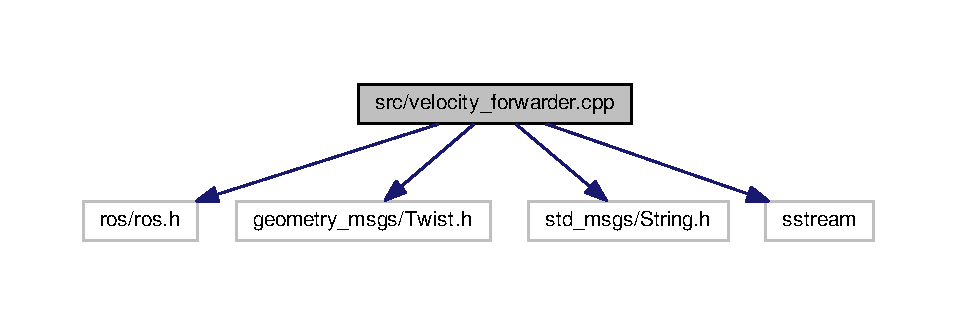
\includegraphics[width=350pt]{velocity__forwarder_8cpp__incl}
\end{center}
\end{figure}
\subsection*{Functions}
\begin{DoxyCompactItemize}
\item 
void \hyperlink{velocity__forwarder_8cpp_a5121f63bb791a335dbb5110dd1afbaa9}{Callback\+\_\+activator1} (const geometry\+\_\+msgs\+::\+Twist \&\hyperlink{velocity__forwarder_8cpp_aba2f97176e275688941f5c2a40324b8a}{msg})
\item 
void \hyperlink{velocity__forwarder_8cpp_aa9ddda9a2dce0b17a19a6b1f8f96e7cb}{Callback\+\_\+activator2} (const geometry\+\_\+msgs\+::\+Twist \&\hyperlink{velocity__forwarder_8cpp_aba2f97176e275688941f5c2a40324b8a}{msg})
\item 
int \hyperlink{velocity__forwarder_8cpp_a3c04138a5bfe5d72780bb7e82a18e627}{main} (int argc, char $\ast$$\ast$argv)
\end{DoxyCompactItemize}
\subsection*{Variables}
\begin{DoxyCompactItemize}
\item 
geometry\+\_\+msgs\+::\+Twist \hyperlink{velocity__forwarder_8cpp_aba2f97176e275688941f5c2a40324b8a}{msg}
\item 
ros\+::\+Publisher \hyperlink{velocity__forwarder_8cpp_a350594df3e8f6948c8462edfd41ce086}{pub}
\end{DoxyCompactItemize}


\subsection{Function Documentation}
\index{velocity\+\_\+forwarder.\+cpp@{velocity\+\_\+forwarder.\+cpp}!Callback\+\_\+activator1@{Callback\+\_\+activator1}}
\index{Callback\+\_\+activator1@{Callback\+\_\+activator1}!velocity\+\_\+forwarder.\+cpp@{velocity\+\_\+forwarder.\+cpp}}
\subsubsection[{\texorpdfstring{Callback\+\_\+activator1(const geometry\+\_\+msgs\+::\+Twist \&msg)}{Callback_activator1(const geometry_msgs::Twist &msg)}}]{\setlength{\rightskip}{0pt plus 5cm}void Callback\+\_\+activator1 (
\begin{DoxyParamCaption}
\item[{const geometry\+\_\+msgs\+::\+Twist \&}]{msg}
\end{DoxyParamCaption}
)}\hypertarget{velocity__forwarder_8cpp_a5121f63bb791a335dbb5110dd1afbaa9}{}\label{velocity__forwarder_8cpp_a5121f63bb791a335dbb5110dd1afbaa9}
The Callback functions, mainly publish the received messages on the topic chosen in the \char`\"{}int main\char`\"{} The only difference, as said before, is the beginning of the display message\+: \char`\"{}\+Subscriber 1 velocities\+:\char`\"{} and \char`\"{}\+Subscriber 2 velocities\+:\char`\"{} R\+O\+S\+\_\+\+I\+N\+F\+O\+\_\+\+S\+T\+R\+E\+AM outputs the received messages through the terminal \index{velocity\+\_\+forwarder.\+cpp@{velocity\+\_\+forwarder.\+cpp}!Callback\+\_\+activator2@{Callback\+\_\+activator2}}
\index{Callback\+\_\+activator2@{Callback\+\_\+activator2}!velocity\+\_\+forwarder.\+cpp@{velocity\+\_\+forwarder.\+cpp}}
\subsubsection[{\texorpdfstring{Callback\+\_\+activator2(const geometry\+\_\+msgs\+::\+Twist \&msg)}{Callback_activator2(const geometry_msgs::Twist &msg)}}]{\setlength{\rightskip}{0pt plus 5cm}void Callback\+\_\+activator2 (
\begin{DoxyParamCaption}
\item[{const geometry\+\_\+msgs\+::\+Twist \&}]{msg}
\end{DoxyParamCaption}
)}\hypertarget{velocity__forwarder_8cpp_aa9ddda9a2dce0b17a19a6b1f8f96e7cb}{}\label{velocity__forwarder_8cpp_aa9ddda9a2dce0b17a19a6b1f8f96e7cb}
\index{velocity\+\_\+forwarder.\+cpp@{velocity\+\_\+forwarder.\+cpp}!main@{main}}
\index{main@{main}!velocity\+\_\+forwarder.\+cpp@{velocity\+\_\+forwarder.\+cpp}}
\subsubsection[{\texorpdfstring{main(int argc, char $\ast$$\ast$argv)}{main(int argc, char **argv)}}]{\setlength{\rightskip}{0pt plus 5cm}int main (
\begin{DoxyParamCaption}
\item[{int}]{argc, }
\item[{char $\ast$$\ast$}]{argv}
\end{DoxyParamCaption}
)}\hypertarget{velocity__forwarder_8cpp_a3c04138a5bfe5d72780bb7e82a18e627}{}\label{velocity__forwarder_8cpp_a3c04138a5bfe5d72780bb7e82a18e627}
We subscribe to the \char`\"{}ac1/cmd\+\_\+vel\char`\"{} and \char`\"{}ac2/cmd\+\_\+vel\char`\"{} topics, which are the topics where the nodes \char`\"{}activator\+\_\+1\char`\"{} and \char`\"{}activator\+\_\+2\char`\"{} publish messages respectively. Everytime we receive a message we will execute the callback functions \char`\"{}\+Callback\+\_\+activator1\char`\"{} and \char`\"{}\+Callback\+\_\+activator2\char`\"{} depending on the topic we receive the incoming message. They both do mainly the same, so we could use the same callback function for both, but we have split them so we can see which topic are we reading from on the terminal.

\subsection{Variable Documentation}
\index{velocity\+\_\+forwarder.\+cpp@{velocity\+\_\+forwarder.\+cpp}!msg@{msg}}
\index{msg@{msg}!velocity\+\_\+forwarder.\+cpp@{velocity\+\_\+forwarder.\+cpp}}
\subsubsection[{\texorpdfstring{msg}{msg}}]{\setlength{\rightskip}{0pt plus 5cm}geometry\+\_\+msgs\+::\+Twist msg}\hypertarget{velocity__forwarder_8cpp_aba2f97176e275688941f5c2a40324b8a}{}\label{velocity__forwarder_8cpp_aba2f97176e275688941f5c2a40324b8a}
\index{velocity\+\_\+forwarder.\+cpp@{velocity\+\_\+forwarder.\+cpp}!pub@{pub}}
\index{pub@{pub}!velocity\+\_\+forwarder.\+cpp@{velocity\+\_\+forwarder.\+cpp}}
\subsubsection[{\texorpdfstring{pub}{pub}}]{\setlength{\rightskip}{0pt plus 5cm}ros\+::\+Publisher pub}\hypertarget{velocity__forwarder_8cpp_a350594df3e8f6948c8462edfd41ce086}{}\label{velocity__forwarder_8cpp_a350594df3e8f6948c8462edfd41ce086}

%--- End generated contents ---

% Index
\backmatter
\newpage
\phantomsection
\clearemptydoublepage
\addcontentsline{toc}{chapter}{Index}
\printindex

\end{document}
